\subsection{Experiments}
\label{sec:congruence_experiments}

In this section, we present the experimental evaluation of our length compression algorithm.
We tested our method on 3965 proofs of problems of the SMT-LIB benchmark.
The proofs were created from problems in the SMT theory QF\_UF, which is the logic of unquantified formulas built over a signature of uninterpreted (i.e. free) sort and function symbols\footnote{QF\_UF specification: \url{http://smtlib.cs.uiowa.edu/logics/QF\_UF.smt2}}, using the SMT solver VeriT \cite{Bouton2009}.
The average length of the proofs is 103450 nodes and the largest proof has length 2241042.

We evaluated the compression achieved by our algorithm for the two different Congruence Graph structures, presented in Section \ref{sec:algorithm}.
We post processed the produced proofs with another compression algorithm called DAGify.
DAGify traverses the proofs and merges duplicate nodes.
This was necessary, because our the congruence compression algorithm creates the same axioms and intermediate nodes multiple times.
A future version of our algorithm should keep track of and reuse nodes, so the post processing is not necessary.
To present unbiased results, we also compressed the proofs with DAGify to show how much of the compression is achieved by this method.

The compression results are presented in Table \ref{tab:congruence_results}, where the rows Equation Graph and Proof Forest display the results of our congruence compression algorithm using the respective type of Congruence Graph.
The row DAGify displays the compression achieved by this algorithm.
\textbf{Compression} was calculated according to Formula \ref{eq:length}, where $f$ is the respective compression algorithm and $B$ denotes the set of benchmark proofs.
The columns \textbf{Min}- and \textbf{Max Compression} show the minimum and maximum compression ratio achieved by the algorithms.
On top of compression, we measure computation speed measured in processed nodes per millisecond.
The best respective results are highlighted in boldface.

\begin{align}
	compression(f) = 1 - \frac{\sum_{\varphi \in B}{\plength{f(\varphi)}}}{\sum_{\varphi \in B}{\plength{\varphi}}}
  \label{eq:length}
\end{align}


%%%%%%%%%%%%%%%%%%%%%%%%%%%%%%%%%%%%%%%%%%%%%%%%%%%%%%%%%%%%%%
%%%%%%%%%%%%%%% Results table %%%%%%%%%%%%%%%%%%%%%%%%%%%%%%%%
%%%%%%%%%%%%%%%%%%%%%%%%%%%%%%%%%%%%%%%%%%%%%%%%%%%%%%%%%%%%%%

\begin{table}[h]
\centering
%\setlength{\tabcolsep}{8pt}
\begin{tabular}{l c c c c}
\toprule
\textbf{Method} & \textbf{Compression} & \textbf{Min Compression} & \textbf{Max Compression} & \textbf{Speed}\\ 
\midrule

Equation Graph & \textbf{5.350} \% & -18.302 \% & \textbf{81.347} \% & 0.343 \\ 
Proof Forest &  5.196 \% & -43.985 \% & 77.202 \% & 0.611 \\ 
DAGify & 3.368 \% & \textbf{0.0} \% & 14.433 \% & \textbf{1.655} \\ 

\bottomrule
%\hline
\end{tabular}
\caption{Compression Results}
\label{tab:congruence_results}
\end{table}

The compression results presented in Table \ref{tab:congruence_results} show that our compression algorithm can achieve an effective compression of roughly 2\%.
This is not really a satisfying number, but the maximum compression for single proofs shows, that our algorithm can perform very well on some examples.
The min compression column shows, that sometimes our method increases the proof length.
However, as seen in Figure \ref{fig:congruence_compression}, this only happens for small proofs.
Figure \ref{fig:congruence_compression} displays the compression achieved by our algorithm, using the Equation Graph data structure, in relation to the proof length.
Every point in the plot represents a proof, where the x-coordinate is its length and the y-coordinate denotes the compression achieved on this proof.
The plot shows that our algorithm has the trend to produce better compression on larger proofs and those are the proofs that are especially interesting for proof compression and in general.

\begin{figure}[h]
	\centering
	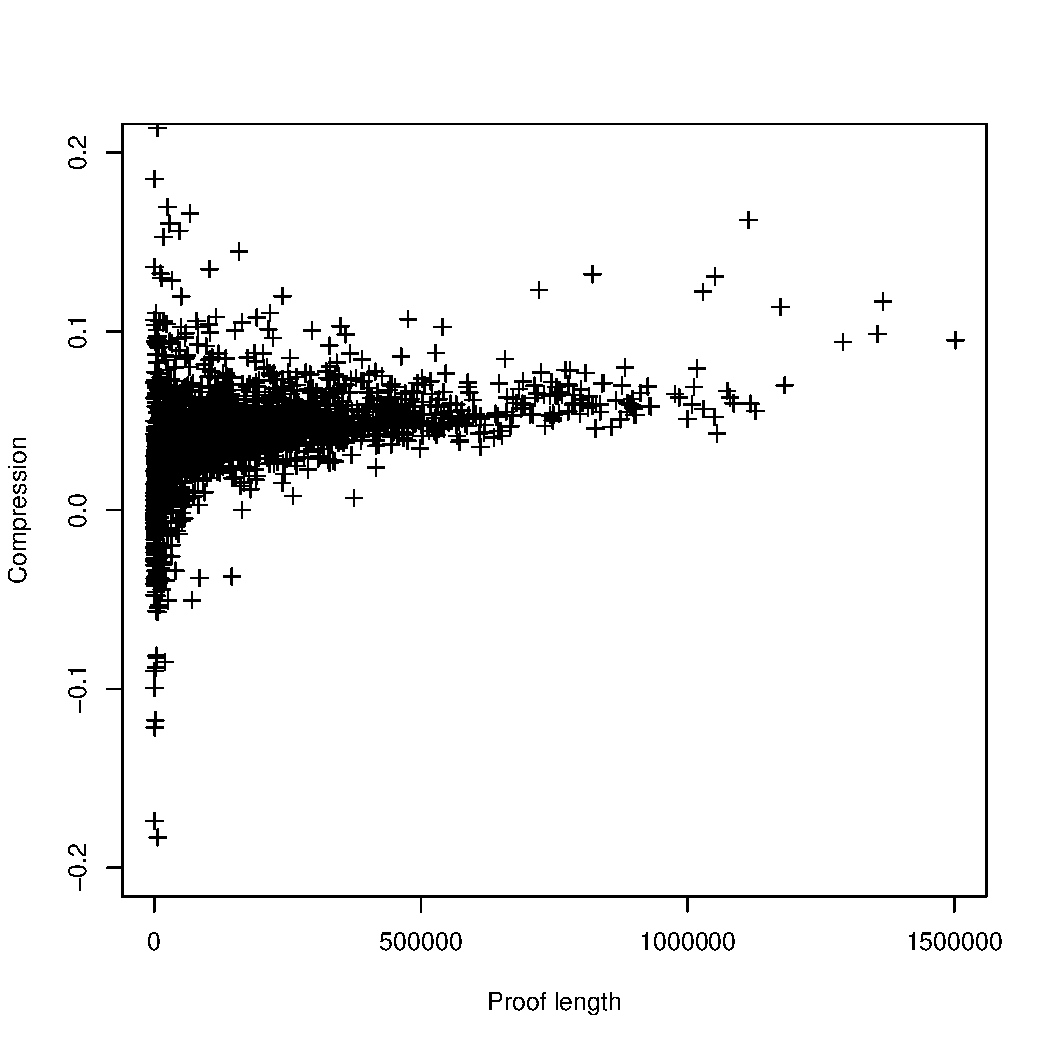
\includegraphics[scale=0.8]{chapters/congruence/figures/compression_vs_length.pdf}
	\caption{Compression vs Proof Length}
	\label{fig:congruence_compression}
\end{figure}

In Section \ref{sec:proofproduction}, we discussed the question on which proof nodes the congruence closure algorithm should be applied to.
For the results presented, the algorithm has been applied to all nodes.
Preliminary experiments showed unpromising results, when the compression algorithm is only applied to low theory lemmas.
A reason could be that the original proofs resolve with input derived nodes early.
The result of such a resolving strategy is that the explanation for some equation is split into multiple nodes or in an input derived node.
In other words, a proof that fulfills the assumption stated in the proof of Proposition \ref{prop:extended_resolution} should contain all explanations in a low theory lemma.
However, proofs created by VeriT do not satisfy this assumption.
Therefore, taking into account equations of ancestor nodes for an explanation in the compression algorithm could improve performance.

On top of proof compression, we measured the explanation sizes produced using the two types Congruence Graphs.
The results are displayed in Table \ref{tab:explanation_results}.
Overall 6604751 explanations were produced by each congruence graph structure.
Of the nodes corresponding to these explanations, 5114638 (77.439 \%) are theory lemmas and 1710435 (25.897\%) are low theory lemmas.
The column \textbf{Compressed} shows the percentage of explanations produced by our algorithm that are strictly smaller than the ones present in the proof.
Note that the produced explanations are at most as large as the original ones by design of the method.
Among the compressed explanations explanations, the column \textbf{Compression} shows the compression ratio achieved, computed according to $1 - \frac{\text{produced}}{\text{original}}$.

%%%%%%%%%%%%%%%%%%%%%%%%%%%%%%%%%%%%%%%%%%%%%%%%%%%%%%%%%%%%%%
%%%%%%%%%%%%%%% Explanation table %%%%%%%%%%%%%%%%%%%%%%%%%%%%
%%%%%%%%%%%%%%%%%%%%%%%%%%%%%%%%%%%%%%%%%%%%%%%%%%%%%%%%%%%%%%

\begin{table}[h]
\centering
%\setlength{\tabcolsep}{8pt}
\begin{tabular}{l c c}
\toprule
\textbf{Congruence Graph} & \textbf{Compressed} & \textbf{Compression} \\ 
\midrule

Equation Graph & 12.42 \% & 28.34 \% \\ 
Proof Forest & 11.459 \% & 28.69 \% \\ 

\bottomrule
%\hline
\end{tabular}
\caption{Explantion Size Results}
\label{tab:explanation_results}
\end{table}

The results show that our explanation producing congruence closure algorithm is able to produce shorter explanations than those of the benchmark proofs often.
The two data structures do not show very significant performance differences and the 1 \% more compressed explanations explain the slight performance edge in proof compression of the Equation Graph over the Proof Forest.

It is surprising that a significant amount of explanations could be compressed by a significant percentage, but still the proof compression achieved is rather small.
The reason probably lies in our proof producing algorithm that produces redundant proofs in some other characteristic than explanation size.
Another reason probably is the combination of fragments of the original proof and newly produced subproofs.
In Section \ref{sec:proofproduction} and Example \ref{example:compressproof} we briefly discussed nodes remaining in the proof when replacing subproofs.
This effect seems to be significant.

However, the results also show that using our congruence closure algorithm within the proof production process in the first place will produce proofs that are even shorter than the ones we are able to obtain by compressing them after creation.
Furthermore, the algorithm can be used in other context where small explanations are desired.